\chapter{Robotersystem}
\label{kap:Robotersystem}
Das Robotersystem beschreibt das Endprodukt dieses Projekts - eine mechanische Einheit mit bipedaler Fortbewegung. Diesbez�glich ist zu beachten, dass keinerlei Autonomie und Intelligenz in dem System steckt. Der Schwerpunkt liegt einzig auf der datenbankbasierten Fortbewegung. \\
Um eine bestm�gliche Bewegungsfreiheit zu gew�hrleisten, muss das mechanische System perfekt mit dem des Menschen �bereinstimmen. Nur dann sind dem Aufzeichnen, sowie dem Konvertieren in Bewegungsfolgen keine Grenzen gesetzt.\\
In diesem Projekt wird das Robotersystem mit manueller Eingabe bewegt, bzw. gesteuert.

\section{Ansteuerung}
\label{kap:Ansteuerung}
Der Aufbau des Gesamtsystem und dessen Funktionsweise ist in Abbildung XXX prinzipiell dargestellt.

\begin{figure}[H]
\centering
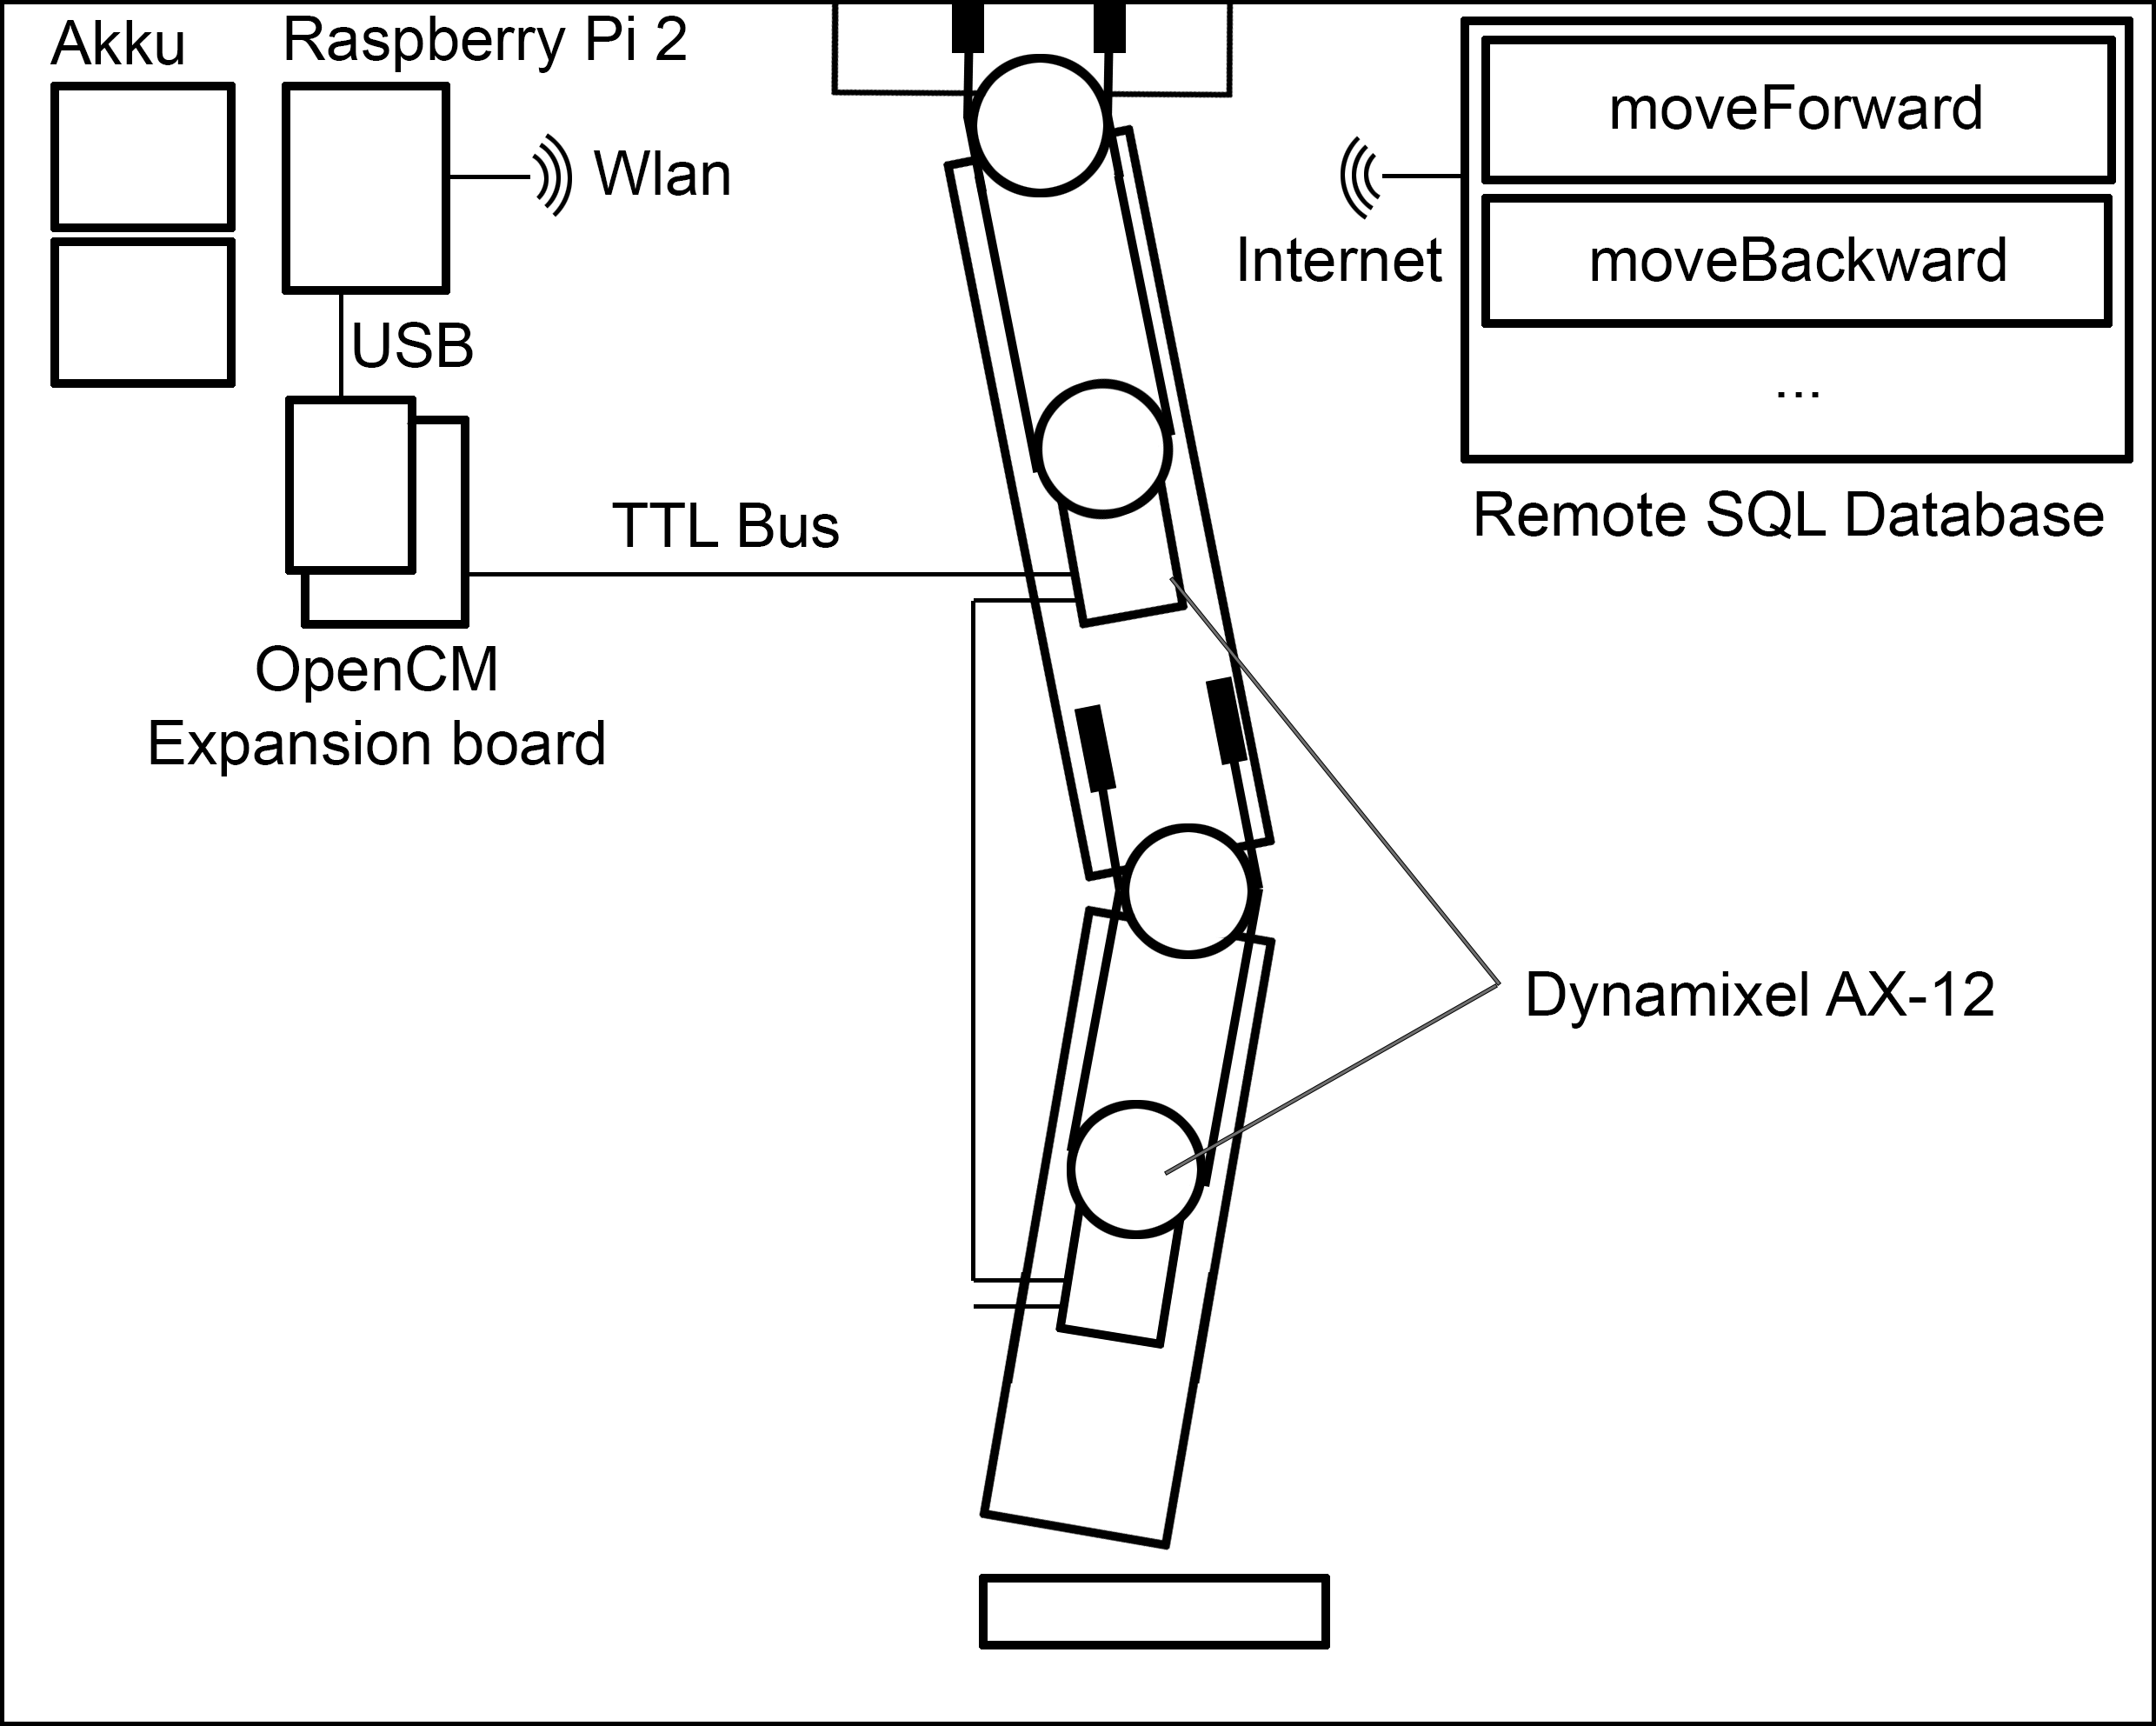
\includegraphics[width=1.0\linewidth]{03_Grafiken/Robotersystem/Aufbau}
\caption[Ansteuerung / Aufbau (Prinzip)]{Ansteuerung / Aufbau (Prinzip)}
\label{fig:aufbau}
\end{figure}

Dabei ist zun�chst das mechanische Modell vernachl�ssigbar, da dieses im weiteren Verlauf Erl�uterung findet. Zun�chst wird die softwaretechnische Seite betrachtet und dessen elektronischen Komponenten, die zur Ansteuerung des Gesamtsystems genutzt werden, erl�utert.\\
Diesbez�glich befindet sich im oberen linken Teil der GRafik die Konstellation der beteiligten Baugruppen und deren Verkn�pfung zueinander. Der Raspberry Pi 2 dient als Steuerzentrale, auf dem das \gls{BS} Windows 10 IOT installiert ist. Darauf ist eine Software aktiv, mit der die gesamte Reglung des Systems abgearbeitet wird. Entsprechend erfolgt das Senden von Befehlen (zur Ansteuerung der Motoren) vom Raspberry Pi aus �ber eine USB-Schnittstelle hin zum OpenCM Board. Dieses Board liest die Befehle und gibt diese an die Motoren (Dynamixel AX-12) weiter. Das Expansion Board ist notwendig, da das OpenCM-Board keine TTL-Schnittstelle zur Verf�gung stellt.\\
Der eigentlich Clou des Systems besteht darin, dass beim Neustart (sofern notwendig) die Bewegungss�tze von einer externen Datenbank heruntergeladen werden. Diesbez�glich verf�gt der Raspberry Pi �ber eine Wlan, bzw. UMTS-Schnittstelle. Die SQL-Datenbank ist �ber das Internet erreichbar, sodass stets aktuelle Bewegungss�tze zur Verf�gung stehen. Die BEwegungss�tze werden mit dem, in Kapitel \ref{kap:Messsystem} beschriebenen Messsystem erstellt / erweitert.
\subsection{Protokoll}
% Sequentielle Block�bertragung f�r max 8 Motoren

\subsection{Testprogramm}
% WriteToComPort

\subsection{Kontrollprogramm}
% MovementControl

\subsection{Clientprogramm}
% Programm auf dem OpenCM
\section{Mechanisches Modell}
\label{kap:MechModell}

\subsection{Prinzipieller Aufbau}

